\documentclass{standalone}
\usepackage{tikz}
\usetikzlibrary{patterns}

\begin{document}
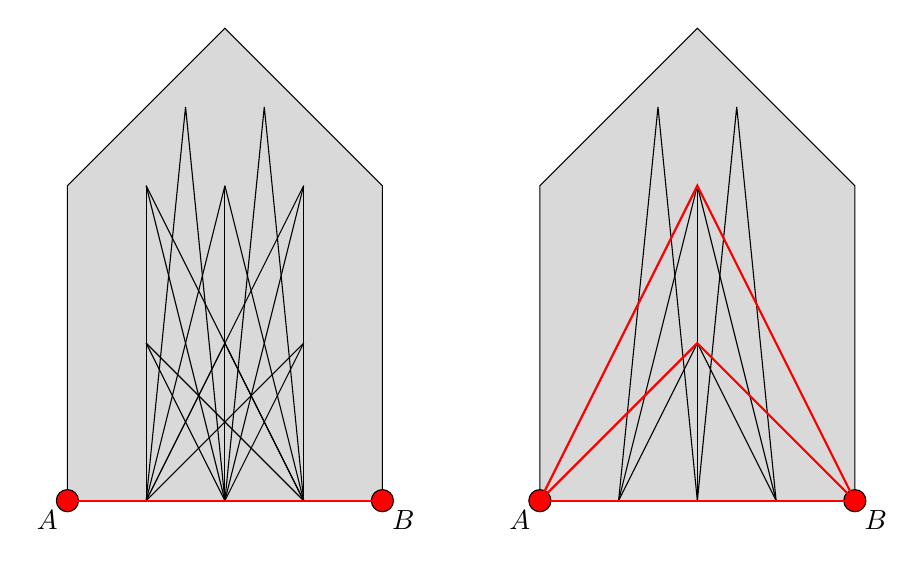
\begin{tikzpicture}
    % Define the coordinates for the polygon vertices
    \coordinate (A) at (0, 0);
    \coordinate (B) at (4, 0);
    \coordinate (C1) at (0, 4);
    \coordinate (C2) at (4, 4);
    
    % Draw the main polygon
    \draw[fill=gray!30] (A) -- (C1) -- (2, 6) -- (C2) -- (B) -- cycle;
    
    % Draw the triangulation lines
    \foreach \x in {1, 2, 3} {
        \foreach \y in {1, 2, 3} {
            \draw (\x, 0) -- (\y, 2);
            \draw (\x, 0) -- (\y, 4);
        }
    }
    \draw (1, 0) -- (1.5, 5) -- (2, 0);
    \draw (3, 0) -- (2.5, 5) -- (2, 0);
    
    % Highlight points A and B
    \draw[fill=red] (A) circle (4pt) node[below left] {$A$};
    \draw[fill=red] (B) circle (4pt) node[below right] {$B$};
    
    % Draw the secant line L
    \draw[red, thick] (A) -- (B);
    
    % Draw the second part of the figure with the cut
    \begin{scope}[xshift=6cm]
        % Redefine coordinates for the second polygon
        \coordinate (A) at (0, 0);
        \coordinate (B) at (4, 0);
        \coordinate (C1) at (0, 4);
        \coordinate (C2) at (4, 4);
        
        % Draw the main polygon
        \draw[fill=gray!30] (A) -- (C1) -- (2, 6) -- (C2) -- (B) -- cycle;
        
        % Draw the triangulation lines
        \foreach \x in {1, 2, 3} {
            \draw (\x, 0) -- (2, 2);
            \draw (\x, 0) -- (2, 4);
        }
        \draw (1, 0) -- (1.5, 5) -- (2, 0);
        \draw (3, 0) -- (2.5, 5) -- (2, 0);
        
        % Highlight points A and B
        \draw[fill=red] (A) circle (4pt) node[below left] {$A$};
        \draw[fill=red] (B) circle (4pt) node[below right] {$B$};
        
        % Draw the secant line L and highlight the triangulation lines from A and B
        \draw[red, thick] (A) -- (B);
        \foreach \y in {2, 4} {
            \draw[red, thick] (A) -- (2, \y) -- (B);
        }
    \end{scope}
\end{tikzpicture}
\end{document}